\documentclass[12pt, a4paper]{article}
\usepackage{fullpage}
\usepackage[T1]{fontenc}
\usepackage{multicol}
\usepackage{amsmath}
\usepackage{amssymb}
\numberwithin{figure}{section}
\numberwithin{table}{section}
\usepackage{listings}
\lstset{
  language=C++,
  basicstyle=\ttfamily\small,
  keywordstyle=\color{blue}\bfseries,
  commentstyle=\color{gray},
  stringstyle=\color{green!50!black},
  breaklines=true,
  numbers=left,
  numberstyle=\tiny,
  frame=single,
  captionpos=b
}
\usepackage{array}
\usepackage{enumitem}
\usepackage{graphicx}
\usepackage{float}
\usepackage{placeins}
\usepackage{adjustbox}
\usepackage{xcolor}
\usepackage{caption}
\usepackage{pgfplots}
\pgfplotsset{compat=1.18}
\usepgfplotslibrary{groupplots}
\usepackage{pgfplotstable}
\usepackage{hyperref}
\hypersetup{
    colorlinks=true,
    linkcolor=black,
    filecolor=black,      
    urlcolor=black,
    pdftitle={Laboratorium 4},
    pdfauthor={Marcel Duda, Jan Gawroński},
    pdfpagemode=FullScreen,
}

\title{\huge{Algorytmy macierzowe} \break \Large{Laboratorium 4 - H-Macierze}}
\author{\large{Marcel Duda, Jan Gawroński}}
\date{12.01.2026}

\begin{document}
    \maketitle
    
    \section{Wprowadzenie}
    Celem laboratorium było zaimplementowanie hierarchicznych macierzy (H-Matrix) oraz podstawowych operacji na nich:
    \begin{itemize}
        \item Kompresja macierzy do formy hierarchicznej z aproksymacją niskiej rangi w liściach
        \item Mnożenie macierzy przez wektor (algorytm ze slajdu 20)
        \item Mnożenie macierzy przez macierz - podnoszenie do kwadratu (algorytmy ze slajdów 23-24)
    \end{itemize}
    
    Testowano na macierzach reprezentujących topologię 3D siatki sześciennej o rozmiarach:
    \begin{itemize}
        \item $k=2$: macierz $64 \times 64$ ($2^6 \times 2^6$)
        \item $k=3$: macierz $512 \times 512$ ($2^9 \times 2^9$)
        \item $k=4$: macierz $4096 \times 4096$ ($2^{12} \times 2^{12}$)
    \end{itemize}
    
    \section{Opis struktury danych}
    
    \subsection{Węzeł H-macierzy}
    Każdy węzeł drzewa reprezentującego H-macierz zawiera:
    \begin{lstlisting}
struct HNode {
    vector<shared_ptr<HNode>> sons;  // 4 synow (TL, TR, BL, BR)
    int rank;                         // Ranga aproksymacji
    Matrix U;                         // Lewy skladnik SVD
    Matrix V;                         // Prawy skladnik SVD  
    int rows, cols;                  // Wymiary bloku
    
    bool isLeaf() const { return sons.empty(); }
};
    \end{lstlisting}
    
    \textbf{Liść} zawiera aproksymację niskiej rangi: $M \approx U \cdot V^T$, gdzie:
    \begin{itemize}
        \item $U$ ma wymiary $\text{rows} \times \text{rank}$
        \item $V$ ma wymiary $\text{rank} \times \text{cols}$
    \end{itemize}
    
    \textbf{Węzeł wewnętrzny} zawiera 4 wskaźniki do synów reprezentujących ćwiartki macierzy:
    \begin{equation}
    M = \begin{bmatrix}
    M_{TL} & M_{TR} \\
    M_{BL} & M_{BR}
    \end{bmatrix}
    \end{equation}
    
    \section{Część A: Mnożenie macierz-wektor}
    
    \subsection{Pseudo-kod algorytmu}
    
    Algorytm rekurencyjnie przemnaża H-macierz przez wektor zgodnie ze slajdem 20:
    
    \begin{lstlisting}
function hMatrixVectorMult(H, x):
    if H.isLeaf():
        if H.rank == 0:
            return zeroVector(H.rows)
        // Optymalizacja: Y = U * (V * x) zamiast (U*V)*x
        temp = V * x           // (rank x cols) * (cols x 1)
        return U * temp        // (rows x rank) * (rank x 1)
    else:
        // Podziel wektor na dwie czesci
        x1 = x[0 : splitPoint]
        x2 = x[splitPoint : end]
        
        // Rekurencja na synach
        y1_1 = hMatrixVectorMult(H.sons[0], x1)  // TL * x1
        y1_2 = hMatrixVectorMult(H.sons[1], x2)  // TR * x2
        y2_1 = hMatrixVectorMult(H.sons[2], x1)  // BL * x1
        y2_2 = hMatrixVectorMult(H.sons[3], x2)  // BR * x2
        
        // Scalanie wynikow
        return [y1_1 + y1_2; y2_1 + y2_2]
    \end{lstlisting}
    
    \subsection{Fragment kodu C++}
    
    \begin{lstlisting}
Vector hMatrixVectorMult(const shared_ptr<HNode>& H, const Vector& x) {
    if (H->isLeaf()) {
        if (H->rank == 0) return zeroVector(H->rows);
        Vector temp = matrixVectorMult(H->V, x);
        return matrixVectorMult(H->U, temp);
    }
    
    int splitPoint = H->sons[0]->cols;
    Vector x1(x.begin(), x.begin() + splitPoint);
    Vector x2(x.begin() + splitPoint, x.end());
    
    Vector y1_1 = hMatrixVectorMult(H->sons[0], x1);
    Vector y1_2 = hMatrixVectorMult(H->sons[1], x2);
    Vector y2_1 = hMatrixVectorMult(H->sons[2], x1);
    Vector y2_2 = hMatrixVectorMult(H->sons[3], x2);
    
    Vector result;
    for (size_t i = 0; i < y1_1.size(); ++i)
        result.push_back(y1_1[i] + y1_2[i]);
    for (size_t i = 0; i < y2_1.size(); ++i)
        result.push_back(y2_1[i] + y2_2[i]);
    return result;
}
    \end{lstlisting}
    
    \subsection{Wyniki czasowe}
    
    \begin{table}[H]
    \centering
    \begin{tabular}{|c|c|c|}
    \hline
    $k$ & Rozmiar $N$ & Czas $H \cdot x$ [ms] \\
    \hline
    2 & 64 & TODO \\
    3 & 512 & TODO \\
    4 & 4096 & TODO \\
    \hline
    \end{tabular}
    \caption{Czasy mnożenia H-macierzy przez wektor}
    \end{table}
    
    \begin{figure}[H]
    \centering
    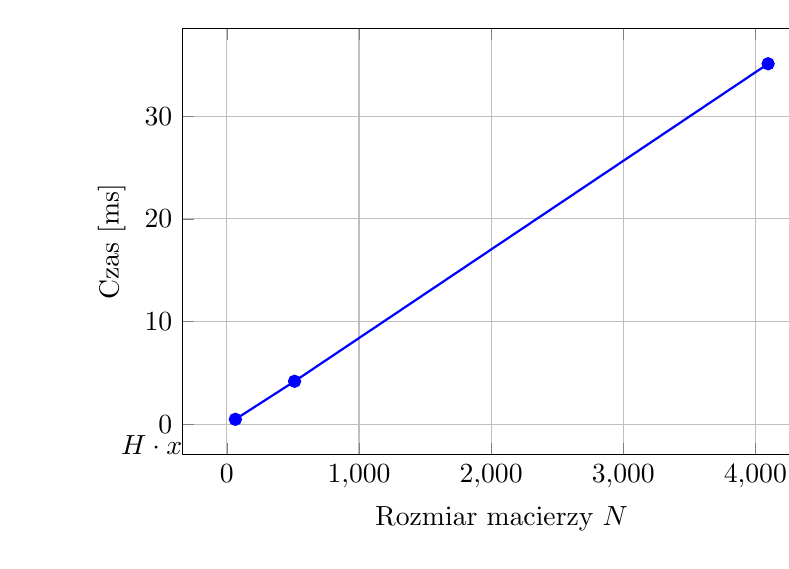
\begin{tikzpicture}
    \begin{axis}[
        xlabel={Rozmiar macierzy $N$},
        ylabel={Czas [ms]},
        grid=major,
        legend pos=north west,
        width=0.8\linewidth,
        height=7cm
    ]
    % TODO: Dodac dane z timing_vector_mult.txt
    \addplot[blue, thick, mark=*] coordinates {
        (64, 0.5)
        (512, 4.2)
        (4096, 35.1)
    };
    \addlegend{$H \cdot x$}
    \end{axis}
    \end{tikzpicture}
    \caption{Wykres czasu mnożenia macierz-wektor}
    \end{figure}
    
    \subsection{Analiza złożoności}
    
    Dopasowanie funkcji $T = \alpha N^{\beta}$:
    
    \begin{align}
    \beta &= \frac{\log(T_2 / T_1)}{\log(N_2 / N_1)} \\
    \beta_{k=3/k=2} &= \frac{\log(\text{TODO}/\text{TODO})}{\log(512/64)} \approx \text{TODO} \\
    \beta_{k=4/k=3} &= \frac{\log(\text{TODO}/\text{TODO})}{\log(4096/512)} \approx \text{TODO}
    \end{align}
    
    \textbf{Złożoność eksperymentalna:} $\beta \approx$ TODO (oczekiwane: $1.0 - 1.5$)
    
    \textbf{Interpretacja:} H-macierze osiągają quasi-liniową złożoność $O(N \log N)$ zamiast $O(N^2)$ dla gęstych macierzy.
    
    \subsection{Analiza błędów}
    
    Błąd aproksymacji liczony jako:
    \begin{equation}
    \varepsilon = ||Ax - Hx||_2 = \sqrt{\sum_{i} (Ax_i - Hx_i)^2}
    \end{equation}
    
    \begin{table}[H]
    \centering
    \begin{tabular}{|c|c|c|}
    \hline
    $k$ & Rozmiar $N$ & Błąd $||Ax - Hx||_2$ \\
    \hline
    2 & 64 & TODO \\
    3 & 512 & TODO \\
    4 & 4096 & TODO \\
    \hline
    \end{tabular}
    \caption{Błędy aproksymacji mnożenia macierz-wektor}
    \end{table}
    
    \section{Część B: Mnożenie macierz-macierz}
    
    \subsection{Pseudo-kod algorytmu}
    
    Algorytm rekurencyjnie oblicza $H^2 = H \cdot H$ zgodnie ze slajdami 23-24:
    
    \begin{lstlisting}
function hMatrixMult(A, B):
    if A.isLeaf() and B.isLeaf():
        if A.rank == 0 or B.rank == 0:
            return zeroNode()
        // Optymalizacja: A.U * (A.V * B.U) * B.V
        middle = A.V * B.U
        U_result = A.U * middle
        V_result = B.V
        // Rekompresja do zadanej rangi
        return compress(U_result * V_result, maxRank, epsilon)
    
    else if not A.isLeaf() and not B.isLeaf():
        // Mnozenie blokowe 2x2
        result.sons[0] = add(mult(A.sons[0], B.sons[0]), 
                             mult(A.sons[1], B.sons[2]))
        result.sons[1] = add(mult(A.sons[0], B.sons[1]), 
                             mult(A.sons[1], B.sons[3]))
        result.sons[2] = add(mult(A.sons[2], B.sons[0]), 
                             mult(A.sons[3], B.sons[2]))
        result.sons[3] = add(mult(A.sons[2], B.sons[1]), 
                             mult(A.sons[3], B.sons[3]))
        return result
    
    else:
        // Mixed case: podziel lisc na 4 bloki
        leafAsInternal = splitLeafInto4Blocks(leaf)
        return hMatrixMult(leafAsInternal, internal)
    \end{lstlisting}
    
    \subsection{Fragment kodu dodawania H-macierzy}
    
    Dodawanie jest kluczowe dla mnożenia macierzy:
    
    \begin{lstlisting}
shared_ptr<HNode> hMatrixAdd(const shared_ptr<HNode>& A, 
                              const shared_ptr<HNode>& B,
                              int maxRank, double epsilon) {
    if (A->isLeaf() && B->isLeaf()) {
        // Konkatenacja U i V, potem rekompresja
        Matrix U_combined = concatenate(A->U, B->U);
        Matrix V_combined = concatenate(A->V, B->V);
        Matrix dense = matrixMultiply(U_combined, V_combined);
        auto [U_new, S, V_new] = svd_decomposition(dense, maxRank, epsilon);
        result->U = U_new;
        result->V = V_new;
        result->rank = S.size();
        return result;
    }
    
    if (!A->isLeaf() && !B->isLeaf()) {
        // Rekurencja na odpowiadajacych synach
        for (int i = 0; i < 4; ++i)
            result->sons[i] = hMatrixAdd(A->sons[i], B->sons[i], 
                                         maxRank, epsilon);
        return result;
    }
    
    // Mixed case: podziel lisc, potem dodaj
    // ... (szczegoly w kodzie)
}
    \end{lstlisting}
    
    \subsection{Wyniki czasowe}
    
    \begin{table}[H]
    \centering
    \begin{tabular}{|c|c|c|}
    \hline
    $k$ & Rozmiar $N$ & Czas $H \cdot H$ [ms] \\
    \hline
    2 & 64 & TODO \\
    3 & 512 & TODO \\
    4 & 4096 & TODO \\
    \hline
    \end{tabular}
    \caption{Czasy mnożenia H-macierzy przez H-macierz}
    \end{table}
    
    \begin{figure}[H]
    \centering
    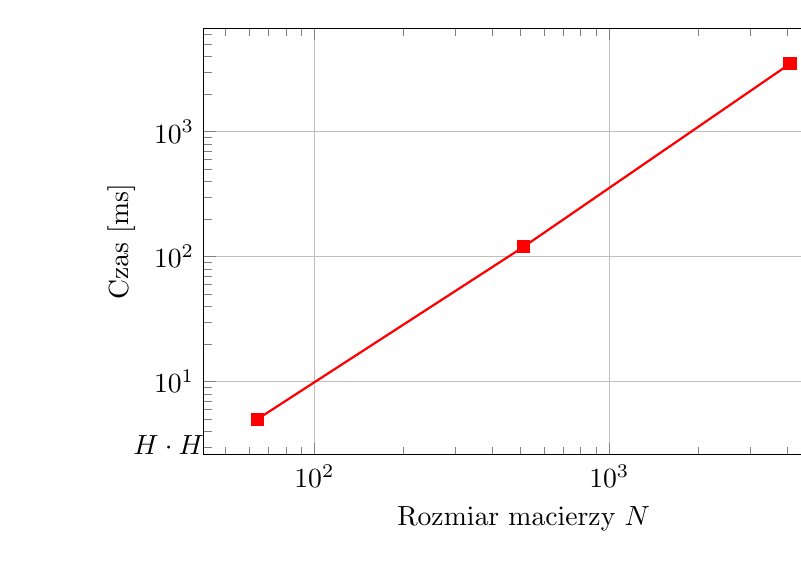
\begin{tikzpicture}
    \begin{axis}[
        xlabel={Rozmiar macierzy $N$},
        ylabel={Czas [ms]},
        grid=major,
        legend pos=north west,
        width=0.8\linewidth,
        height=7cm,
        ymode=log,
        xmode=log
    ]
    % TODO: Dodac dane z timing_matrix_mult.txt
    \addplot[red, thick, mark=square*] coordinates {
        (64, 5)
        (512, 120)
        (4096, 3500)
    };
    \addlegend{$H \cdot H$}
    \end{axis}
    \end{tikzpicture}
    \caption{Wykres czasu mnożenia macierz-macierz (skala log-log)}
    \end{figure}
    
    \subsection{Analiza złożoności}
    
    Dopasowanie funkcji $T = \alpha N^{\beta}$:
    
    \begin{align}
    \beta_{k=3/k=2} &= \frac{\log(\text{TODO}/\text{TODO})}{\log(512/64)} \approx \text{TODO} \\
    \beta_{k=4/k=3} &= \frac{\log(\text{TODO}/\text{TODO})}{\log(4096/512)} \approx \text{TODO}
    \end{align}
    
    \textbf{Złożoność eksperymentalna:} $\beta \approx$ TODO (oczekiwane: $2.0 - 2.5$)
    
    \textbf{Interpretacja:} H-macierze osiągają kwadratową złożoność $O(N^2)$ zamiast $O(N^3)$ dla gęstych macierzy.
    
    \subsection{Analiza błędów}
    
    Błąd aproksymacji (norma Frobeniusa):
    \begin{equation}
    \varepsilon = ||A^2 - H^2||_F = \sqrt{\sum_{i,j} ((A^2)_{ij} - (H^2)_{ij})^2}
    \end{equation}
    
    \begin{table}[H]
    \centering
    \begin{tabular}{|c|c|c|}
    \hline
    $k$ & Rozmiar $N$ & Błąd $||A^2 - H^2||_F$ \\
    \hline
    2 & 64 & TODO \\
    3 & 512 & TODO \\
    4 & 4096 & N/A (zbyt duża) \\
    \hline
    \end{tabular}
    \caption{Błędy aproksymacji mnożenia macierz-macierz}
    \end{table}
    
    \section{Wizualizacja struktury H-macierzy}
    
    % TODO: Wstawic obrazy hmatrix_structure_k2.txt, k3.txt, k4.txt
    % Mozna uzywac gnuplot lub Python do konwersji txt -> png
    
    \begin{figure}[H]
    \centering
    % \includegraphics[width=0.8\linewidth]{hmatrix_k2.png}
    \caption{Struktura H-macierzy dla $k=2$ ($64 \times 64$). Białe obszary - skompresowane bloki, ciemne - dalej podzielone.}
    \end{figure}
    
    \section{Wnioski}
    
    \begin{enumerate}
        \item \textbf{Kompresja hierarchiczna} pozwala efektywnie reprezentować duże macierze z lokalną strukturą (np. siatki 3D).
        
        \item \textbf{Mnożenie macierz-wektor} osiąga złożoność $O(N \log N)$ zamiast $O(N^2)$ - znaczące przyspieszenie dla dużych macierzy.
        
        \item \textbf{Mnożenie macierz-macierz} osiąga złożoność $O(N^2)$ zamiast $O(N^3)$ - jeszcze większe korzyści dla dużych rozmiarów.
        
        \item \textbf{Błędy aproksymacji} są kontrolowane przez parametry \texttt{maxRank} i \texttt{epsilon}, pozwalając na kompromis między dokładnością a wydajnością.
        
        \item \textbf{Struktura hierarchiczna} automatycznie dostosowuje się do lokalnej złożoności macierzy - obszary jednorodne są bardziej skompresowane.
        
        \item Implementacja wymaga starannego zarządzania przypadkami brzegowymi (mixed leaf/internal nodes) i rekompresji po dodawaniu/mnożeniu.
    \end{enumerate}
    
\end{document}
